\section{Capacity-limited native search preserves a strong allocation rule}
\label{sec:native-capacity}
\subsection{A separate activity objective under original production laws}
The preceding count/content search does not identify a useful objective-to-system
distinction. We therefore conduct a separately declared native pilot with
existing capacity limits, not a retrospective change of its losses. Five
original Qwen3-8B university researchers operate for four years over the same
103,107-record corpus, with base30 balanced resources. The original
\code{papers\_per\_project}=2 cap permits partial submissions. Fixed funding
at fraction0.2 supplies one total annual award slot across programs. Native
research cost remains10 when an active researcher has a working project;
the original per-paper flow has no direct submission debit. Neither a paper
fee nor a new resource law is activated to force a trade-off.

Alongside $T=-A$, let $I_{iy}$ be one exactly when founder$i$ is author-capable
and has\code{is\_active}=true at the end of year$y$, and zero otherwise.
Define the separate loss
\[
 P=-\sum_{y=1}^{4}\sum_{i\in F} I_{iy},
\]
where $F$ is the initial five-researcher cohort. New actors do not enlarge
the cohort. The formal minimum is$-20$; the indicator does not certify
resource sufficiency, useful work or continuous survival. In particular,
native zero-resource activity semantics are preserved. P is an objective
in its own search, not an additional constraint on T or an adoption veto.
Every complete world receives both scores from its original checkpoints.

Five common developer rules precede two own slots per objective at explicitly
reused development seed61001. All rules use their declared native authority:
reviewed accept-all with equalization; its transfer cut; no-review accept-all
with equalization; and reviewed accept-all with reserve-proximity or
completion-priority allocation. The latter rules conserve resources and seek
a pre-cost reserve of21. They are strong hand controls, not generated inventions.
Each actual editing parent minimizes the assigned loss over common references
and its own history; all four slots start from reserve-proximity. Final selection
is instead restricted to complete own literal submissions, including retention,
with the earliest tie and no reference fallback. The local35B designer has
16 proposal steps per slot and64 optional historical component probes.
Initial and four history-bearing technical calibrations precede dispatch.

\subsection{All submissions, strong ties and a real execution failure}
All four slots submit literal programs. Three complete native execution;
P/g1 fails and receives neither a numerical loss nor a replacement. Both
original cold audits and cost projections agree, as do two exports of each
score, effect, input and preference analysis.
Table~\ref{tab:capacity-all} retains the full comparison.

\begin{table}[t]
\centering\small
\begin{tabular}{lrrl}
\toprule
System or own slot & T & P & Annual active founders\\
\midrule
Reviewed all / equalization & $-10$ & $-12$ & 5,5,1,1\\
Reviewed all / transfer cut & $-10$ & $-12$ & 4,4,2,2\\
No-review all / equalization & $-10$ & $-12$ & 5,5,1,1\\
Reviewed all / reserve-proximity & $-12$ & $-15$ & 5,5,3,2\\
Reviewed all / completion-priority & $-12$ & $-15$ & 5,5,3,2\\
T/g0; selected T & $-12$ & $-15$ & 5,5,3,2\\
P/g0; selected P & $-12$ & $-15$ & 5,5,3,2\\
P/g1 & --- & --- & Technical null after year2\\
T/g1; ties T/g0 & $-12$ & $-15$ & 5,5,3,2\\
\bottomrule
\end{tabular}
\caption{All nine physical attempts in the capacity pilot. Lower losses are
better. The failed world has two saved annual boundaries and recorded work
in year3, not a completed four-year outcome. Equal sums for the first three
rules conceal different activity paths. All complete own submissions tie
both strong allocation rules; there is no generated-policy advantage.}
\label{tab:capacity-all}
\end{table}

No own submission changes nodes, connections or schedules. T/g0 replaces
the already all-accept selection source with unconditional acceptance and
constant final score1. T/g1 retains the mean native review score while
rewriting unconditional acceptance. P/g0 likewise retains that mean and
replaces direct field access in the allocation code with existing-value
defaults. These literal edits do not establish a new allocation algorithm.
The full scientist input sequences of P/g0, T/g1 and both strong allocation
references are identical at this observed history, with identical literal
response choices; full provider envelopes are not identical. T/g0 has a
different full input sequence despite the same T/P and activity path.
Observed input equality is not program equivalence on all possible states.

P/g1 attempts a different operation. Its final allocation code includes
initial-founder support and a virtual-source fallback. In year3 it emits
two transfers of10 from the nonexistent actor\code{system}. The native
conserving-transfer receiver rejects the batch because endpoints must be
existing author-capable actors. The original code result and two committed
annual boundaries are retained; partial work is not promoted to a complete
loss. This is an authored invalid command, not evidence that the framework
silently repaired the institution or that the policy performed poorly on P.
Four component probes of that final artifact had returned on historical
fixtures. Their success did not certify the later native consumer or its
trajectory: local code return and valid downstream scientific execution
are distinct tests.

\begin{figure}[t]
\centering
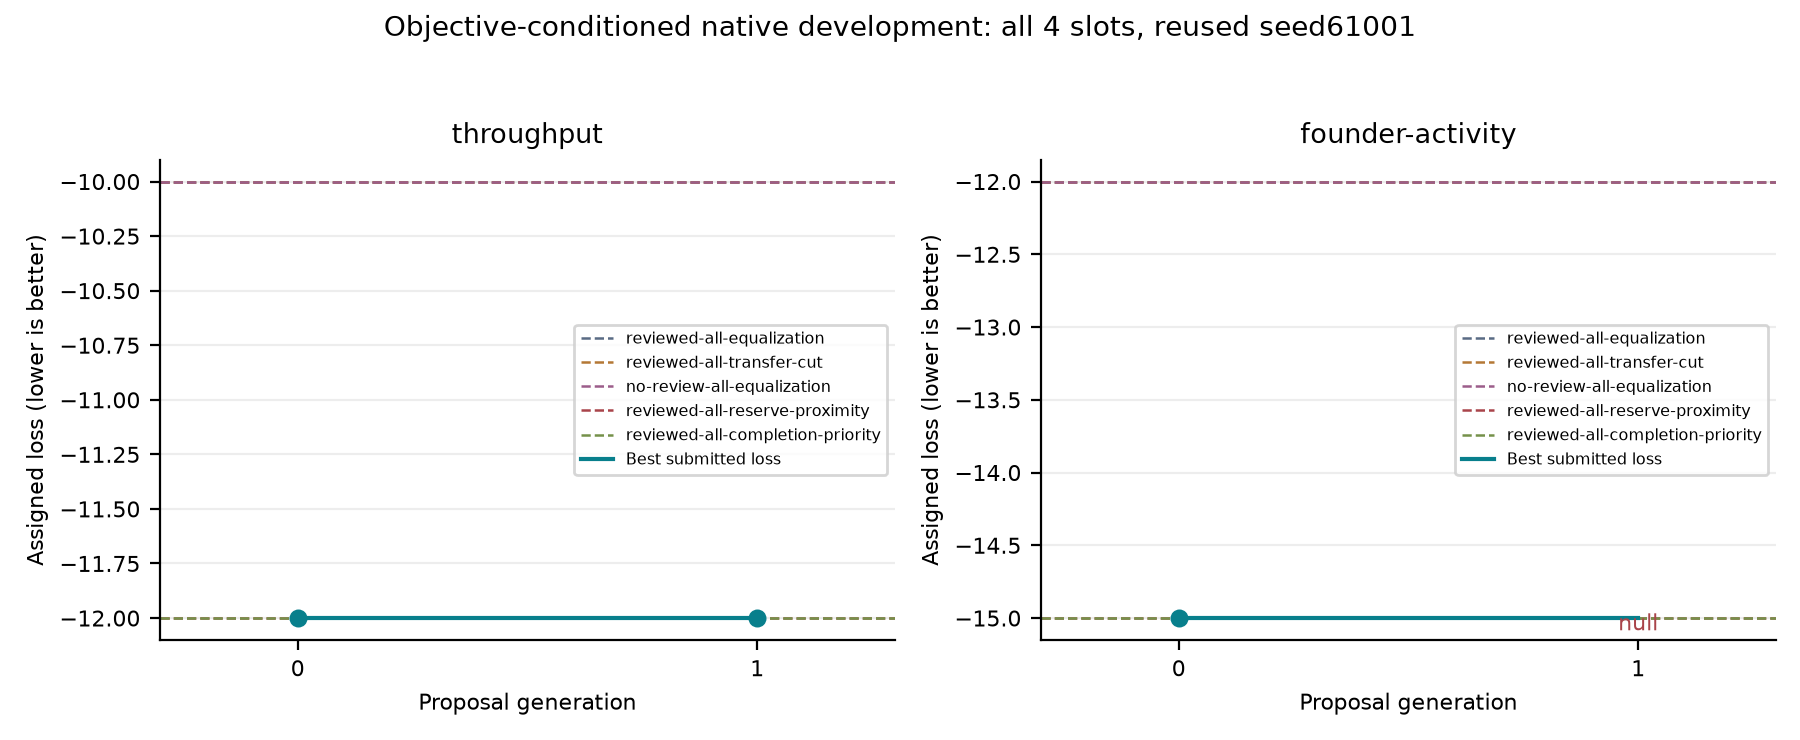
\includegraphics[width=\linewidth]{figures/native-capacity-objective-loop-v1/objective-loss-paths.png}
\caption{Both actual objective-conditioned search paths, all five coincident
reference labels and the P/g1 null. The first own proposal already ties the
strong editing parent; the flat path is not an improvement from that parent.
There is one design history per objective, not independent optimizer replication.}
\label{fig:capacity-paths}
\end{figure}

\subsection{What the common score point does and does not explain}
The eight complete worlds have only two observed score pairs:
$(-12,-15)$ for the two strong controls and three own submissions, and
$(-10,-12)$ for the other three controls. The first strictly dominates the
second in both recorded coordinates. Consequently, every hypothetical
raw-unit linear mixture $wT+(1-w)P$, $0\leq w\leq1$, has the same minimizing
score group in this archive (Figure~\ref{fig:capacity-geometry}). This is an
exact finite-record calculation, not optimization at an interior weight,
a global Pareto frontier or evidence that T and P are intrinsically aligned.
The search did not explore materially different complete organizing systems.

\begin{figure}[t]
\centering
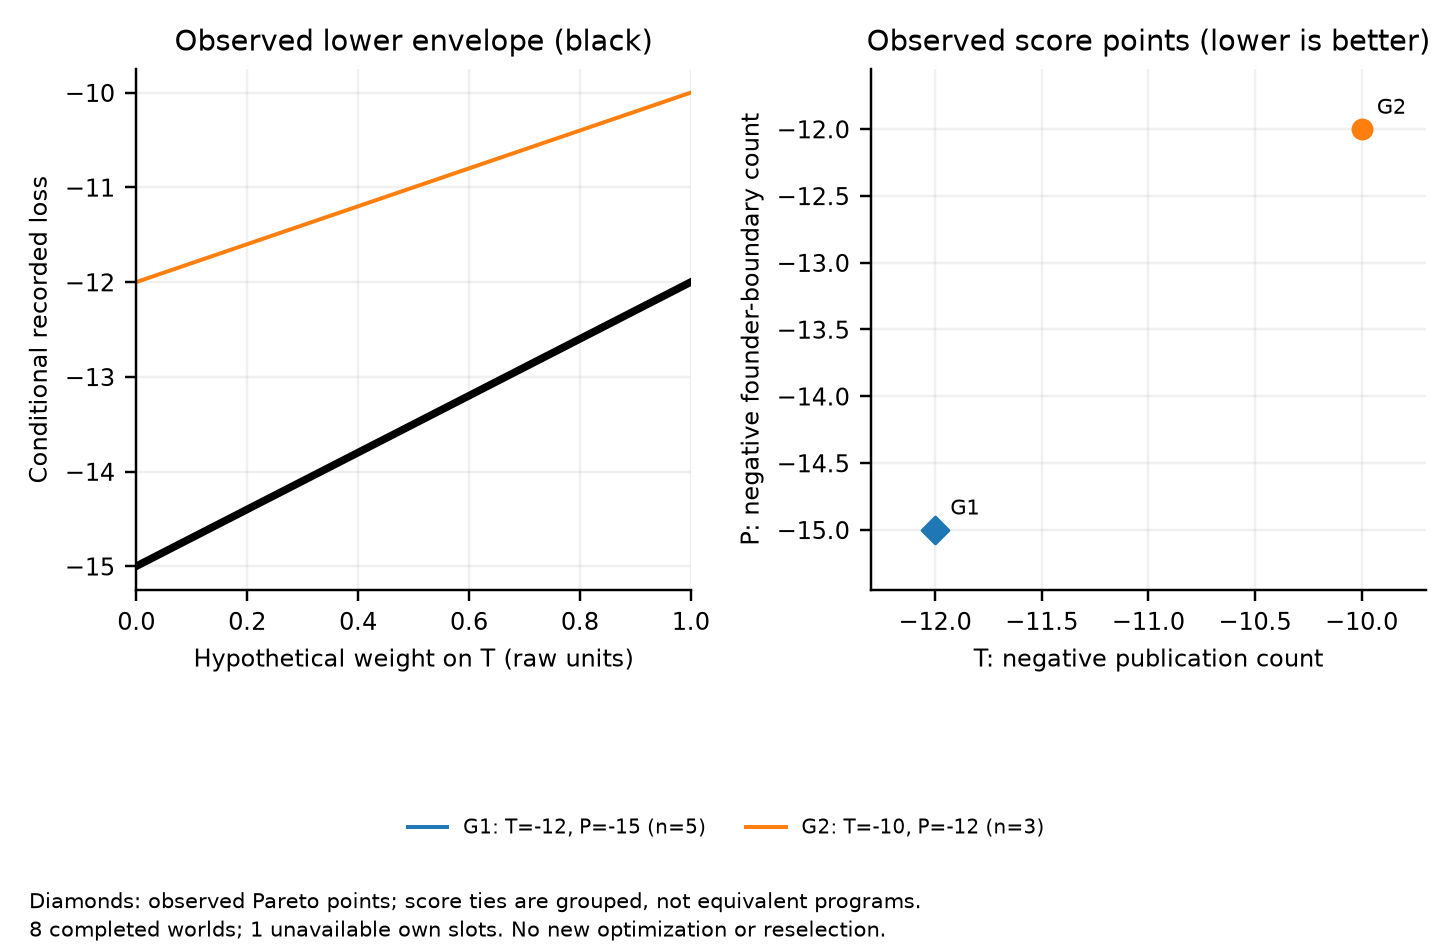
\includegraphics[width=.94\linewidth]{figures/native-capacity-objective-loop-v1/observed-tp-geometry.png}
\caption{Conditional geometry of the complete capacity archive, including
all tied programs and excluding the one null from numerical coordinates.
The lower envelope selects the same score group across raw-unit weights.
Five worlds at one point are neither equivalent programs nor independent
optimizer histories. No new objective, candidate selection or inference is
introduced by this readout.}
\label{fig:capacity-geometry}
\end{figure}

The lower-loss hand rules and own programs have12 rather than10 accepted
decisions and15 rather than12 saved founder boundaries in this development
condition. That comparison concerns allocation rules; it is not evidence of
autonomous invention or a causal mediation estimate for a particular transfer.
The original traces include172 code calls and34 committed annual boundaries,
including the failed prefix. Recorded scientist cost is1,171 completed replies,
1,117,703 input and111,959 output tokens, with213,168 cached input tokens as a
subset. Separate designer transport records contain58 proposal POSTs and142
readiness POSTs;18 role loads have unknown token usage. No critic is called.
Execution takes about2h12min, with cold/reader closure about4min17s later.

We retain this finite negative search result rather than expanding it until
a desired institution wins. The prepared unused-seed evaluator is not
dispatched for this flat pilot: no unused seed has been selected or scored.
The remaining research question is how to obtain and explain a nontrivial
objective-to-system relationship, distinguishing the explored behavior,
designer interface, world dynamics and objective incentives. More fixed-policy
seeds alone would not answer that question or establish publication readiness.
\FloatBarrier
